% Options for packages loaded elsewhere
\PassOptionsToPackage{unicode}{hyperref}
\PassOptionsToPackage{hyphens}{url}
%
\documentclass[
]{article}
\title{contact information}
\author{}
\date{\vspace{-2.5em}}

\usepackage{amsmath,amssymb}
\usepackage{lmodern}
\usepackage{iftex}
\ifPDFTeX
  \usepackage[T1]{fontenc}
  \usepackage[utf8]{inputenc}
  \usepackage{textcomp} % provide euro and other symbols
\else % if luatex or xetex
  \usepackage{unicode-math}
  \defaultfontfeatures{Scale=MatchLowercase}
  \defaultfontfeatures[\rmfamily]{Ligatures=TeX,Scale=1}
\fi
% Use upquote if available, for straight quotes in verbatim environments
\IfFileExists{upquote.sty}{\usepackage{upquote}}{}
\IfFileExists{microtype.sty}{% use microtype if available
  \usepackage[]{microtype}
  \UseMicrotypeSet[protrusion]{basicmath} % disable protrusion for tt fonts
}{}
\makeatletter
\@ifundefined{KOMAClassName}{% if non-KOMA class
  \IfFileExists{parskip.sty}{%
    \usepackage{parskip}
  }{% else
    \setlength{\parindent}{0pt}
    \setlength{\parskip}{6pt plus 2pt minus 1pt}}
}{% if KOMA class
  \KOMAoptions{parskip=half}}
\makeatother
\usepackage{xcolor}
\IfFileExists{xurl.sty}{\usepackage{xurl}}{} % add URL line breaks if available
\IfFileExists{bookmark.sty}{\usepackage{bookmark}}{\usepackage{hyperref}}
\hypersetup{
  pdftitle={contact information},
  hidelinks,
  pdfcreator={LaTeX via pandoc}}
\urlstyle{same} % disable monospaced font for URLs
\usepackage[margin=1in]{geometry}
\usepackage{graphicx}
\makeatletter
\def\maxwidth{\ifdim\Gin@nat@width>\linewidth\linewidth\else\Gin@nat@width\fi}
\def\maxheight{\ifdim\Gin@nat@height>\textheight\textheight\else\Gin@nat@height\fi}
\makeatother
% Scale images if necessary, so that they will not overflow the page
% margins by default, and it is still possible to overwrite the defaults
% using explicit options in \includegraphics[width, height, ...]{}
\setkeys{Gin}{width=\maxwidth,height=\maxheight,keepaspectratio}
% Set default figure placement to htbp
\makeatletter
\def\fps@figure{htbp}
\makeatother
\setlength{\emergencystretch}{3em} % prevent overfull lines
\providecommand{\tightlist}{%
  \setlength{\itemsep}{0pt}\setlength{\parskip}{0pt}}
\setcounter{secnumdepth}{-\maxdimen} % remove section numbering
\ifLuaTeX
  \usepackage{selnolig}  % disable illegal ligatures
\fi

\begin{document}
\maketitle

\hypertarget{uxcc3euxc544uxc624uxb294-uxae38}{%
\subsubsection{찾아오는 길}\label{uxcc3euxc544uxc624uxb294-uxae38}}

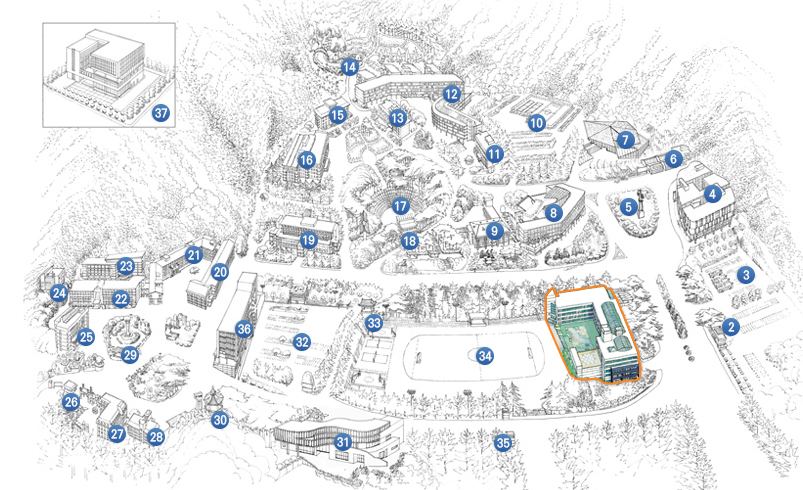
\includegraphics{images/figure5.png}

\textbf{연구실 위치} - 대전광역시 서구 배재로 155-40(도마동)
배재21세기관 P342호

\textbf{찾아오는 길}

\begin{enumerate}
\def\labelenumi{\arabic{enumi})}
\item
  둔산시외버스터미널 → 둔산 CGV 앞 선사유적지 정류장 301번 버스 (10개
  정류장 이동) → 배재대학교 정류장 하차 (약 24분)
\item
  둔산고속버스터미널 → 102번 버스 → 216번 버스
\end{enumerate}

\begin{verbatim}
둥지아파트 정류장까지 도보 약 7분 → 둥지아파트 정류장 102번 버스 승차 (1개 정류장 이동) → 정부청사역 정류장 하차 → 정부청사정류장 216번 버스 승차 (10개 정류장 이동) → 배재대학교 정류장 하차 (약 46분)
\end{verbatim}

\begin{enumerate}
\def\labelenumi{\arabic{enumi})}
\setcounter{enumi}{2}
\item
  대전유성터미널 → 유성시외버스 정류장 312번 버스 승차 (15개 정류장
  이동) → 배재대학교 정류장 하차 (약 47분)
\item
  대전서부터미널 → 도마교 정류장 도보 9분 → 도마교 정류장 312번 버스
  승차 (6개 정류장 이동) → 배재대학교 정류장 하차 (약 33분)
\item
  대전복합터미널 → 601번 버스 → 612번 버스
\end{enumerate}

\begin{verbatim}
복합터미널 정류장 도보 약 6분 → 복합터미널 정류장 601번 버스 승차 (9개 정류장 이동) → 태평오거리 정류장 하차 → 태평오거리 정류장 612번 버스 승차 (12개 정류장 이동) → 배재대학교 정류장 하차 (약 56분)
\end{verbatim}

\begin{enumerate}
\def\labelenumi{\arabic{enumi})}
\setcounter{enumi}{5}
\tightlist
\item
  대전역 → 대전역 정류장 613번 버스 승차 (18개 정류장 이동)
\end{enumerate}

\begin{verbatim}
변동중학교 정류장 하차 → 배재대학교 도보 약 10분 (약 51분)
\end{verbatim}

\begin{enumerate}
\def\labelenumi{\arabic{enumi})}
\setcounter{enumi}{6}
\tightlist
\item
  서대전역 → 버스 이용 (612번 버스)
\end{enumerate}

\begin{verbatim}
서대전역 정류장 도보 약 4분 → 서대전역 정류장 612번 버스 (18개 정류장 이동) → 경남아파트 정류장 하차 (약 39분)
\end{verbatim}

\begin{enumerate}
\def\labelenumi{\arabic{enumi})}
\setcounter{enumi}{7}
\tightlist
\item
  택시 이용 (약 34분) 10,900원
\end{enumerate}

\hypertarget{uxc5f0uxad6cuxc2e4-uxc5f0uxb77duxcc98}{%
\subsubsection{연구실
연락처}\label{uxc5f0uxad6cuxc2e4-uxc5f0uxb77duxcc98}}

\begin{verbatim}
042-520-5348 
\end{verbatim}

\end{document}
